\textbf{PROBLEMA 3}
\vspace{20px}

En el circuito de la figura, los valores de las resistencias son $R_1 = 1\,\Omega$ y $R_2 = 100\,\Omega$. Sin embargo,
desconocemos la fuerza electromotriz de la fuente de tensión y la capacidad del condensador. Suponga en todo
momento que la fuente de tensión es ideal (su resistencia interna es despreciable).

\begin{enumerate}[label=\alph*.]
    \item Suponga que, inicialmente, el condensador está completamente descargado. En un momento determinado,
    situamos el interruptor en la posición $A$, conectando la fuente $\mathcal{E}$ y formando un circuito $RC$ con la
    resistencia $R_1$ y el condensador. Con un osciloscopio, medimos el voltaje entre las placas del condensador
    en función del tiempo, $v_C (t)$ y obtenemos, para los instantes previos y posteriores a la conexión de la
    fuente, la curva de la figura. Sabiendo que cada división del eje vertical representa 5\,V, deduzca la fuerza
    electromotriz de la fuente explicando brevemente su razonamiento.
    \item Desconocemos la capacidad del condensador, pero en el laboratorio solo tenemos condensadores de tres
    capacidades, 5\,$\mu$F, 5\,mF y 5\,F, por lo que el condensador del circuito debe ser alguno de estos tres. Sabiendo
    que cada división del eje horizontal de la gráfica representa 5\,s, deduzca la capacidad del condensador
    empleado en el circuito, explicando brevemente su razonamiento.
    \item Suponga que mantenemos el interruptor en la posición $A$ durante un tiempo muy largo, de modo que
    el condensador se carga por completo. En un instante posterior, al que nos referiremos como $t = 0$,
    cambiamos el interruptor a la posición $B$, desconectando la fuente de tensión y conectando el condensador
    a la resistencia $R_2$. Encuentre la expresión para la corriente que circula por la resistencia $R_2$ en función
    del tiempo para $t > 0$.
    \item Si mantenemos el interruptor en la posición $B$ durante un tiempo indefinido, calcule, por el procedimiento
    que considere más adecuado, la energı́a total que disipa la resistencia $R_2$ entre $t = 0$ y $t\;$\rightarrow$ \infty$.
\end{enumerate}

\begin{center}
    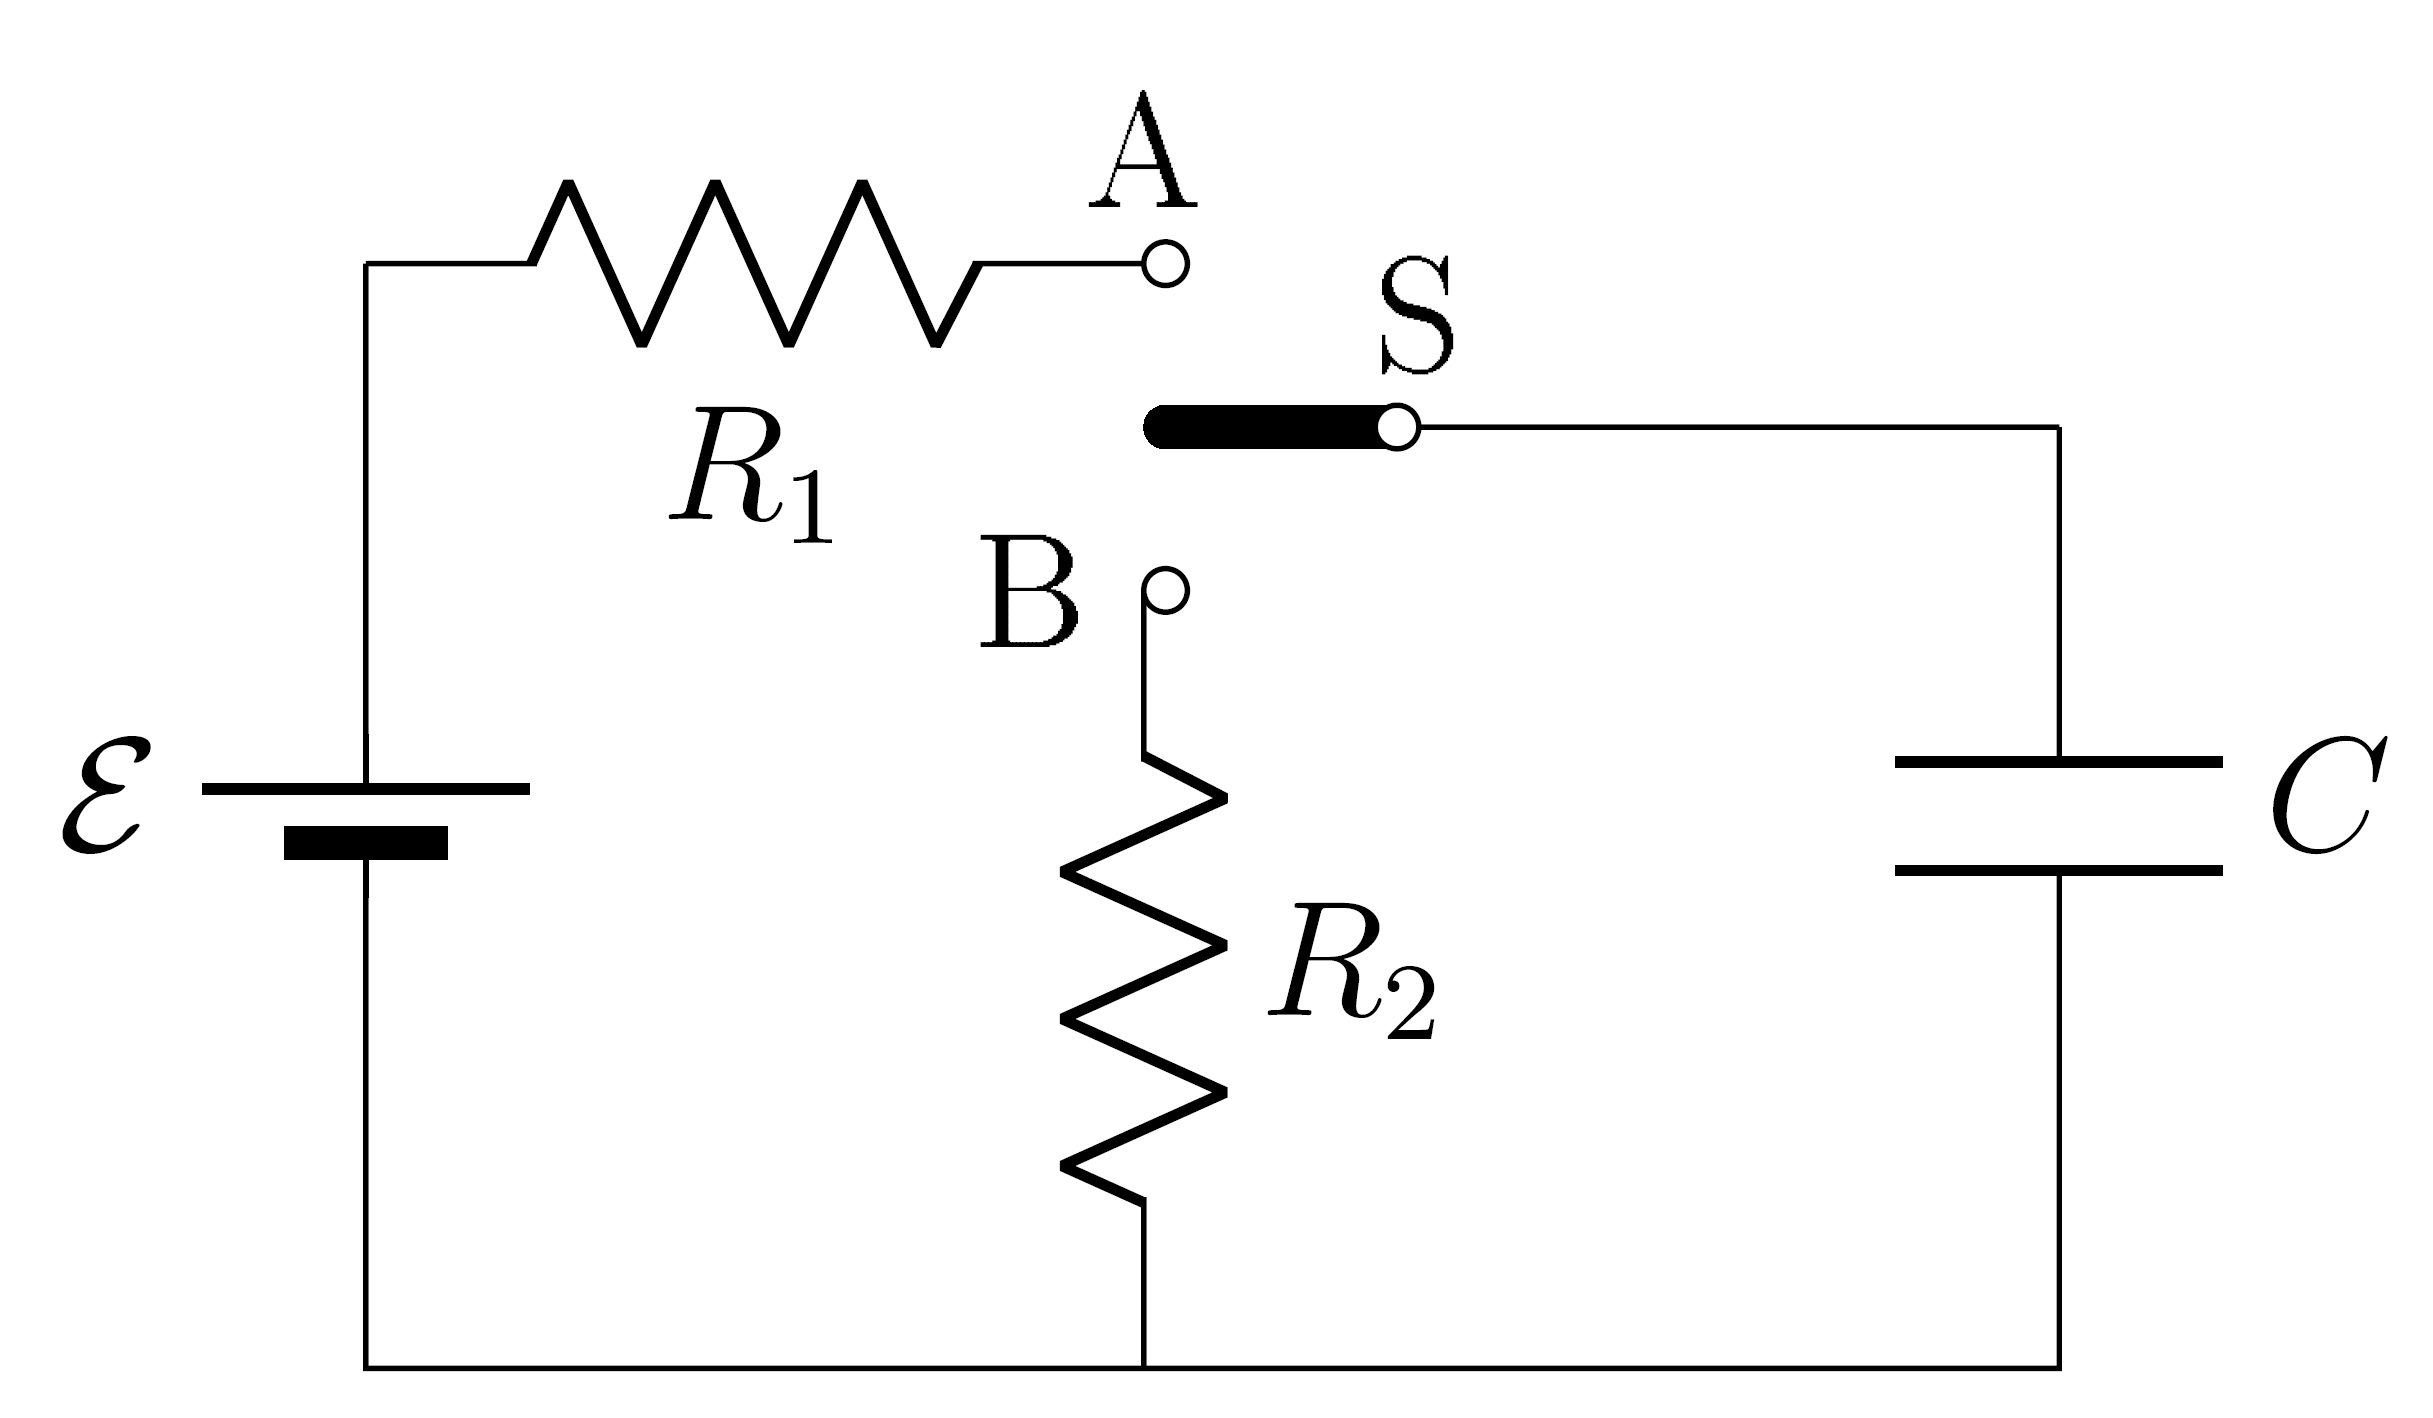
\includegraphics[width=12cm]{files/img3}
\end{center}
\begin{center}
    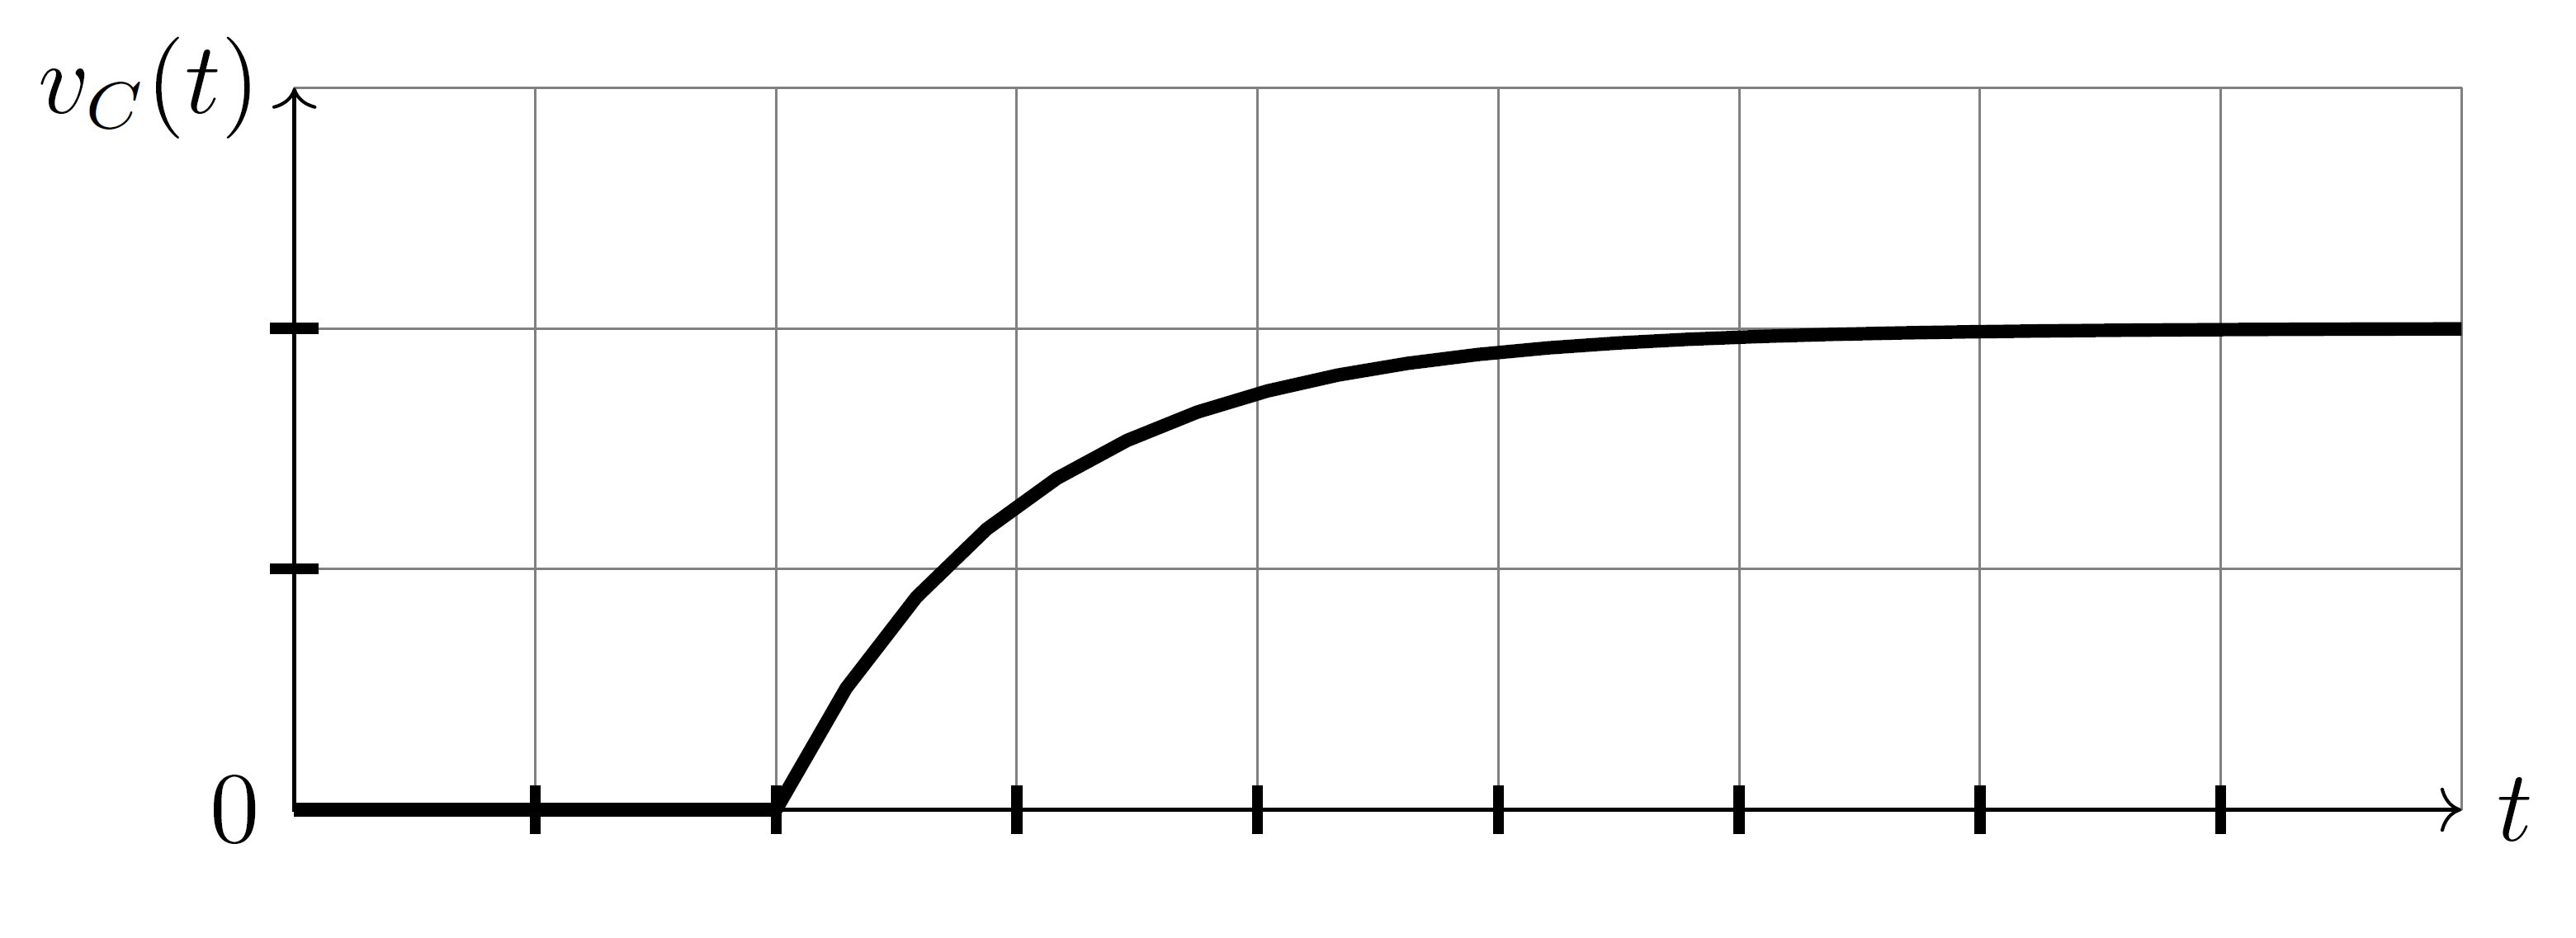
\includegraphics[width=12cm]{files/img4}
\end{center}

\vspace{20px}
\textit{Solución:}
\\

\textbf{a}. En el momento en que se sitúa el interruptor en la posición A, la carga comienza a fluir inmediatamente a través de la
resistencia $R_1$, depositándose en la placa positiva del condensador. A partir de ese momento, la corriente va disminuyendo y la
carga del condensador aumentando, hasta que $I$ es igual a 0 y el voltaje en el condensador, según la regla de las mallas de Kirchhoff,
es $\mathcal{E}$.\\

Por lo tanto, la fuerza electromotriz $\mathcal{E}$  de la fuente es 10 V.

\vspace{20px}
\textbf{b}. Si aplicamos la regla de las mallas de Kirchhoff al circuito, tenemos que:

\begin{equation*}
    \mathcal{E} - R_1 \frac{dQ}{dt} - \frac{Q}{t} = 0
\end{equation*}

Esta es una ecuación diferencial lineal de primer orden, cuya solución es $Q(t) = \mathcal{E} C(1 - e^{- t / R_1 C})$.
Como la capacidad de un condensador no depende de la carga ni el voltaje, podemos obtener una expresión del voltaje del condensador
en función del tiempo:


\begin{equation*}
    V_C(t) = \mathcal{E}(1 - e^{- t / R_1 C})
\end{equation*}

En la gráfica, observamos que para $t \simeq 3.5$\,s, el voltaje en el condensador es aproximadamente la mitad del voltaje final.
Sustituyendo estos valores
en la fórmula anterior y despejando $C$, obtenemos un valor de $5.05$\,F, por lo que el condensador del circuito es el de 5 F.\\

\vspace{20px}
\textbf{c}. En el momento en el que se cambia el interruptor a la posición B, existe una diferencia de potencial entre los extremos de $R_2$,
por lo que debe pasar una corriente por la misma. Esta corriente es:

\begin{equation*}
    I_0 = \frac{\mathcal{E}}{R_2} = \frac{Q_0}{R_2 C}
\end{equation*}

La aplicación de la regla de las mallas de Kirchhoff a este circuito nos da la expresión:

\begin{equation*}
    \frac{Q}{C} - I R_2 = 0
\end{equation*}

La intensidad $I$ se relaciona con la carga $Q$ por la expresión:

\begin{equation*}
    I = - \frac{dQ}{dt}
\end{equation*}

donde el signo menos indica que como $Q$ decrece, $dQ / dt$ es una cantidad negativa. Por tanto, para la carga de este circuito tenemos
una ecuación diferencial expresada como:


\begin{equation*}
    \frac{Q}{C} + R_2 \frac{dQ}{dt} = 0
\end{equation*}

Su solución es $Q(t) = Q_0 e^{-t/R_2 C}$. Derivando esta expresión, obtenemos:

\begin{equation*}
    I(t) = - \frac{dQ(t)}{dt} = \frac{Q_0}{R_2 C} e^{-t/R_2 C} = I_0 e^{-t/R_2 C}
\end{equation*}

\vspace{20px}
\textbf{d}. Podemos calcular la potencia disipada en la resistencia $R_2$ considerando la definición de potencia como la variación
de la energía térmica disipada en la resistencia.

\begin{equation*}
    \frac{d W_{R}}{dt} = I^2 R_2 = \left( \frac{\mathcal{E}}{R_2} e^{-t/R_2 C} \right)^2 R_2 = \frac{\mathcal{E}^2}{R_2}  e^{-2t/R_2 C}
\end{equation*}

Integrando la expresión anterior entre $t = 0$ y $t\;$\rightarrow$ \infty$:

\begin{equation*}
    \int_0^{\infty} \frac{\mathcal{E}^2}{R_2}  e^{-2t/R_2 C} =
    \frac{\mathcal{E}^2}{R_2} \int_0^{\infty}  e^{-2t/R_2 C} =
    \frac{\mathcal{E}^2}{R_2} \frac{R_2 C}{(-2)} e^{-2t/R_2 C} \Big|_0^\infty =
    - \frac{\mathcal{E}^2 C}{2}(0 - 1) = \frac{\mathcal{E}^2 C}{2} = \frac{Q^2}{2 C}
\end{equation*}

Podríamos haber llegado al mismo resultado considerando que toda la energía que posee el condensador antes de que el interruptor
cambie a la posición (B) se disipa en la resistencia $R_2$, y que la energía del condensador en ese momento es la mitad de la proporcionada
por la fuente, $QV = \frac{Q^2}{C}$.